% FactIndic - IEEE conference paper (IEEEtran, 2-column).
% Build:  cd paper && tectonic main.tex        (or: latexmk -xelatex main.tex; XeTeX is needed)
% Word:   python paper/make_docx.py   (IEEE Word layout, see paper/README.md)
% Sections live in sections/*.tex; figures are made by
%   python -m src.analysis.make_figures   (writes paper/figures/*.pdf|png)
\documentclass[conference]{IEEEtran}
\IEEEoverridecommandlockouts

\usepackage{cite}
\usepackage{amsmath}
\usepackage{newtxtext,newtxmath}  % Times, as in IEEE proceedings
\usepackage{graphicx}
\usepackage{booktabs}
\usepackage{multirow}
\usepackage{xcolor}
\usepackage{url}
\usepackage[hidelinks]{hyperref}

\graphicspath{{figures/}}

% Devanagari words in the text (XeTeX/tectonic): \dev{बाढ़}
% Font: fonts/NotoSerifDevanagari-Regular.ttf (SIL Open Font License, fonts/OFL.txt),
% loaded with a plain XeTeX \font command so newtx (Times) is left untouched.
\font\devfont="[fonts/NotoSerifDevanagari-Regular.ttf]:script=deva" at 9pt
\newcommand{\dev}[1]{{\devfont #1}}

% Visible markers for unfinished parts. Search for "TODO" before submission.
\newcommand{\todo}[1]{\textcolor{red}{\textbf{[TODO:} #1\textbf{]}}}
\newcommand{\cond}[1]{\textsc{#1}}   % condition names: \cond{hi}, \cond{hi-rom}, \cond{hinglish}

\begin{document}

\title{FactIndic: Factual Consistency of LLM Summaries\\for Hindi, Romanized Hindi and Hinglish}

\author{
\IEEEauthorblockN{Arman Sahni, Ananya Mishra, Gauri Mahajan, Krati Khanna, Arushi Chakraborty}
\IEEEauthorblockA{\textit{Department of Computer Science and Engineering}, \textit{Bennett University}, Greater Noida, India\\
\{s24cseu1430, s24cseu1431, s24cseu1435, s24cseu0024, s24cseu1269\}@bennett.edu.in}
}

\maketitle

\begin{abstract}
Large language models (LLMs) are increasingly used to summarize news in Indian languages, yet their factual consistency is rarely measured outside English, and almost never for code-mixed Hindi-English (Hinglish), the register in which much of India writes online. We present FactIndic, a training-free study of factual consistency in LLM summaries of 186 BBC Hindi articles from XL-Sum, each presented in three parallel forms: Devanagari Hindi, a rule-based Romanized transliteration (same words, different script) and an LLM-generated Hinglish rewrite (same facts, code-mixed; mean CMI 17.6). We summarize every article with a plain prompt and a factuality-aware prompt using a 4B open model (gemma3:4b, run locally), and compare against a 120B model (gpt-oss-120b) on a 50-article subset. Summaries are evaluated with script-independent number and entity precision/recall, SummaC-style NLI, ROUGE and BERTScore, and 60 summaries are labelled by five annotators. The small model answers in the wrong language or script in up to 9.1\% of Hinglish summaries, while the large model never does. Number and entity precision stay at or above 0.97 in every condition, so explicit hallucination of names and numbers is rare; the factuality-aware prompt instead raises number recall from 0.23 to 0.56 for Hindi. NLI disagrees with the other metrics on the prompt effect, and none of the automatic metrics detects relation errors in which correct names and numbers are combined wrongly. Annotators judge 57\% of the labelled small-model summaries to contain an error (20\% a major one), most often a wrong relation between correct facts, with fair agreement (Fleiss' $\kappa$ = 0.38 for faithful vs.\ error). No automatic metric separates faithful from erroneous summaries better than chance: AUC is 0.49 and 0.39 for the two NLI variants and at most 0.60 (ROUGE-L) for the others, with every 95\% interval including 0.5.
\end{abstract}

\begin{IEEEkeywords}
summarization, factual consistency, hallucination, Hindi, code-mixing, Hinglish, large language models, evaluation
\end{IEEEkeywords}

\section{Introduction}

Abstractive summaries written by neural models often contain statements that the source does not support~\cite{maynez2020faithfulness,ji2023survey}. For news, these \emph{factual inconsistencies} matter more than fluency: a summary that names the wrong winner of a match or reverses who condemned whom is worse than no summary. Large language models (LLMs) now produce fluent summaries in many languages without task-specific training, but most evidence about their faithfulness, and most of the metrics used to measure it, comes from English~\cite{pagnoni2021frank,honovich2022true}.

Hindi is spoken by several hundred million people, and online it is often not written in its native Devanagari script at all. Much everyday writing is \emph{Hinglish}: Hindi grammar in Roman letters, mixed with English words. A summarizer deployed for Indian users will therefore meet three kinds of input for the same content: Devanagari Hindi, Romanized Hindi, and code-mixed Hinglish. Each of them stresses a model differently, and each stresses the \emph{evaluation} differently: named-entity recognizers, NLI models and lexical metrics are typically built for one script and one language at a time.

This paper asks three questions:
\begin{enumerate}
  \item Does the \emph{form} of the input (script, code-mixing) change how faithful LLM summaries are?
  \item Does a factuality-aware prompt, which tells the model to copy names and numbers exactly and add nothing, make summaries more faithful than a plain prompt?
  \item Which automatic metrics can be trusted for this setting, and what do they miss?
\end{enumerate}

To separate the effect of the script from the effect of code-mixing, we build a \emph{parallel} dataset. For each of 186 Hindi news articles from XL-Sum~\cite{hasan2021xlsum} we have the original Devanagari text (\cond{hi}), a deterministic Romanized transliteration that changes only the script (\cond{hi-rom}), and an LLM rewrite into Hinglish that keeps every name, number and sentence (\cond{hinglish}). Because the facts are identical across the three versions, differences in the summaries can be attributed to the input form.

We make the following contributions:
\begin{itemize}
  \item A parallel Hindi / Romanized Hindi / Hinglish dataset of 186 news articles with automatic fact-preservation checks and a measured Code-Mixing Index~\cite{das2014identifying}.
  \item A training-free evaluation pipeline that works across scripts: number matching on parsed values (including Hindi number words such as \emph{teen hazaar} or \emph{dedh crore}), entity matching on a phonetic skeleton that makes Devanagari and Roman spellings comparable, and SummaC-style NLI~\cite{laban2022summac} with two premise granularities.
  \item A controlled comparison of a plain and a factuality-aware prompt for a small local model (gemma3:4b, 1,116 summaries), and a comparison with a 120B model on a 50-article subset, including how often each model answers in the wrong language or script.
  \item A five-annotator human evaluation of 60 summaries with an error typology, used to test which automatic metrics agree with human judgments. \todo{one sentence on the human-label result.}
\end{itemize}

All code, prompts, model outputs and scores are released.\todo{repository URL}

\section{Related Work}

\subsection{Summarization for Indian languages}
XL-Sum~\cite{hasan2021xlsum} collects professionally written BBC article--summary pairs in 44 languages, including Hindi, and reports fine-tuned mT5~\cite{xue2021mt5} baselines. The IndicNLG benchmark~\cite{kumar2022indicnlg} adds summarization and other generation tasks for eleven Indic languages. Both benchmarks evaluate mainly with ROUGE~\cite{lin2004rouge}, which rewards overlap with a reference but does not check whether a summary is supported by its source. mFACE~\cite{aharoni2023mface} is among the few studies of factual consistency in multilingual summarization; it uses an NLI-based consistency model to filter and control training data across XL-Sum languages. We study prompted LLMs rather than fine-tuned models, and add script and code-mixing as controlled factors.

\subsection{Code-mixing}
Code-mixed Hindi-English is common on Indian social media and is challenging for standard NLP pipelines. GLUECoS~\cite{khanuja2020gluecos} collects code-switched benchmarks, including Hindi-English tasks, and shows that models trained on monolingual data degrade on them. The amount of mixing in a text is usually quantified with the Code-Mixing Index (CMI)~\cite{das2014identifying,gamback2016comparing}, which is 0 for monolingual text and rises towards 50 as the two languages are used equally. Summarization of code-mixed text has been studied mainly for conversations: GupShup~\cite{mehnaz2021gupshup} provides Hinglish dialogue--summary pairs. To our knowledge, factual consistency of summaries of code-mixed \emph{news} has not been measured, nor has the effect of script alone been separated from the effect of code-mixing.

\subsection{Factual consistency evaluation}
Maynez et al.~\cite{maynez2020faithfulness} showed that a large share of abstractive summaries contain hallucinated content, and FRANK~\cite{pagnoni2021frank} proposed a typology of factual errors (e.g.\ entity, predicate and circumstance errors) together with human judgments to benchmark metrics. Existing metrics fall into several families:
\begin{itemize}
  \item \emph{Entailment classifiers.} FactCC~\cite{kryscinski2020factcc} trains a classifier on synthetically corrupted summary sentences. SummaC~\cite{laban2022summac} instead applies an off-the-shelf NLI model at the sentence level and aggregates the scores, overcoming the mismatch between document-length premises and sentence-level NLI training data.
  \item \emph{Question answering.} QAGS~\cite{wang2020qags} and QAFactEval~\cite{fabbri2022qafacteval} generate questions from the summary and compare the answers obtained from the summary and from the source.
  \item \emph{Entity-level checks.} Nan et al.~\cite{nan2021entity} measure the precision of named entities in the summary with respect to the source, a simple and interpretable signal of entity hallucination.
\end{itemize}
The TRUE benchmark~\cite{honovich2022true} found NLI- and QA-based metrics to be the strongest on English data. QA-based metrics need question generation and answering models, which are not readily available for Romanized or code-mixed Hindi, so we rely on a multilingual NLI model trained on XNLI-style data~\cite{conneau2018xnli,laurer2024less} and on script-independent entity and number checks in the spirit of Nan et al.

\section{Dataset}
\label{sec:dataset}

\subsection{Source articles}
We start from the Hindi test split of XL-Sum~\cite{hasan2021xlsum} (8,847 BBC Hindi articles, each with a one-sentence reference summary). We keep articles of 150--500 words (5,610 articles) so that every article fits the context of a small model, and draw a random sample of 300 (seed 42). All text is normalized (Unicode NFC, unified dashes and quotation marks, collapsed whitespace).

\subsection{Three parallel conditions}
Each article is presented in three forms that share the same facts:
\begin{itemize}
  \item \cond{hi}: the original Devanagari text.
  \item \cond{hi-rom}: a rule-based Romanized transliteration of the same Hindi words (ITRANS scheme, lowercased, with deletion of the word-final inherent vowel and normalization of nukta letters). No LLM is involved, so only the \emph{script} changes.
  \item \cond{hinglish}: a rewrite into Roman-script Hinglish by gpt-oss-120b~\cite{openai2025gptoss} at temperature 0. The prompt (with four few-shot examples) asks for Hindi grammar with the everyday nouns, verbs and adjectives that urban speakers say in English, requires every name, number, date and unit to stay unchanged, and forbids adding, removing or summarizing content. Relative to \cond{hi-rom}, this adds \emph{code-mixing}.
\end{itemize}

\subsection{Quality control}
Every Hindi--Hinglish pair is checked automatically. All numbers (Devanagari and ASCII digits) are extracted from both versions and compared as multisets, and the Hinglish/Hindi word-count ratio must lie between 0.7 and 1.5. Of the first 189 generated pairs, 180 passed; all nine failures came from number words turned into digits (e.g.\ ``three-D'' written as ``3D''). Each failing pair was regenerated once with the checker's complaint added to the prompt; six were fixed and three were dropped. Generation stopped after 189 articles because of the provider's daily token limit; since the sample order is random, the resulting 186 articles remain a random sample.

\subsection{Code-mixing}
We measure the Code-Mixing Index~\cite{das2014identifying}, $\mathrm{CMI} = 100\,(1 - \max(n_{en}, n_{hi}) / (n_{en} + n_{hi}))$, where $n_{en}$ and $n_{hi}$ count English and Hindi tokens. Tokens are tagged by rule: capitalized words inside a sentence are treated as named entities and ignored; words in a list of common Romanized Hindi words are Hindi; words with an English Zipf frequency $\geq 3$ in \texttt{wordfreq} are English; everything else is Hindi. In a five-article pilot, few-shot examples raised the mean CMI of the rewrites from 6.2 to 13.4. Table~\ref{tab:dataset} summarizes the final dataset.

\begin{table}[t]
\centering
\caption{The FactIndic dataset (186 parallel articles).}
\label{tab:dataset}
\begin{tabular}{@{}lr@{}}
\toprule
Articles (XL-Sum Hindi test, 150--500 words) & 186 \\
Words per article, \cond{hi} (mean $\pm$ sd) & 275.7 $\pm$ 82.1 \\
Words per article, \cond{hinglish} (mean $\pm$ sd) & 276.8 $\pm$ 82.2 \\
Words per reference summary (mean) & 26.8 \\
CMI, \cond{hinglish} (mean/median/range) & 17.6/17.0/1.4--33.3 \\
Named entities per article (Stanza, mean) & 8.7 \\
Distinct numbers per article (mean) & 3.9 \\
Articles without any number & 19 \\
\bottomrule
\end{tabular}
\end{table}

\section{Method}
\label{sec:method}

\subsection{Prompts}
We compare two zero-shot prompts, each applied to all three conditions:
\begin{itemize}
  \item \textbf{Plain}: ``Summarize the following article in 2--3 sentences.''
  \item \textbf{Factual}: the same instruction plus six rules: use only information stated in the article; copy names of people, places and organizations exactly; copy every number, date and amount exactly; add no background knowledge, opinions or guesses; do not translate between English and Hindi in code-mixed text; leave out any fact you are unsure about.
\end{itemize}
Both prompts name the required output language explicitly (Hindi in Devanagari script, Hindi in Roman script, or Hinglish in Roman script) before and after the article. In a pilot, the generic instruction ``use the same language and script as the article'' produced the wrong language in 8 of 18 summaries, mostly English; with an explicit language, 17 of 18 were correct.

\subsection{Models}
The main model is \textbf{gemma3:4b}~\cite{gemma2025gemma3}, a 4-billion-parameter open model that runs on a laptop. It summarizes every article in every condition with both prompts (186 $\times$ 3 $\times$ 2 = 1,116 summaries). As a large-model reference we use \textbf{gpt-oss-120b}~\cite{openai2025gptoss} on the first 50 articles of the (random) sample, for \cond{hi} and \cond{hinglish} with both prompts (200 summaries). No model is trained or fine-tuned.

\subsection{Language/script check}
A summary in the wrong language cannot be compared with its source by lexical or entity metrics, so every summary is first checked automatically. \cond{hi} summaries must be at least 80\% Devanagari letters. \cond{hi-rom} and \cond{hinglish} summaries must be at most 20\% Devanagari, and at most 60\% of their words may be tagged English by the CMI tagger. The 0.6 threshold separates our data cleanly: all Romanized and Hinglish \emph{source} articles score at most 0.33 and English summaries score 0.74--0.96. Wrong-language summaries are kept and reported as a result, but excluded from the factuality metrics.

\subsection{Factual consistency metrics}

\paragraph{Numbers}
We extract numbers from digits (including Devanagari digits and thousands separators) and from number words in both scripts, after transliterating to Roman, e.g.\ \emph{teen hazaar} $\to$ 3000, \emph{dedh crore} $\to 1.5\times10^7$, \emph{700 arab} $\to 7\times10^{11}$. With $N_s$ and $N_d$ the sets of values in the summary and the source document,
\begin{equation}
P_{num} = \frac{|N_s \cap N_d|}{|N_s|}, \qquad R_{num} = \frac{|N_s \cap N_d|}{|N_d|}.
\end{equation}
$P_{num} < 1$ signals an invented or altered number; $R_{num}$ measures how many of the source's numbers are kept. $P_{num}$ is undefined for summaries without numbers and is then left out of the averages.

\paragraph{Entities}
Gold entities are obtained with Stanza~\cite{qi2020stanza} Hindi NER on the Devanagari article. To match names across scripts we map every word to a \emph{phonetic skeleton}: it is transliterated to Roman, similar sounds are merged (ph/f, sh/s, w/v, z/j, aspiration dropped), and non-initial vowels are removed, so that ``Stansted'', its Devanagari spelling and the transliteration ``stainasted'' all become \texttt{stnstd}. Two skeletons match if their \texttt{rapidfuzz} partial ratio is at least 85. This threshold was set on 20 hand-labelled (entity, summary) pairs sampled across score bands, where it classifies 19 of 20 correctly (80: 17/20; 90: 13/20). Entity recall counts the gold entities found in the summary, over those gold entities that can be found in that condition's source (the Hinglish rewrite occasionally translates an organization name). Entity precision checks summary entities against the source: Stanza entities for Devanagari summaries, runs of capitalized words for Roman-script summaries.

\paragraph{NLI}
Following SummaC-ZS~\cite{laban2022summac}, each summary sentence $s$ is scored by an NLI model against premises $p$ drawn from the source, and receives $\max_p P(\textit{entail}\mid p, s)$; the summary score is the mean over its sentences, and sentences scoring below 0.5 are counted as unsupported. We use mDeBERTa-v3-base~\cite{he2023debertav3} fine-tuned on multilingual NLI data~\cite{laurer2024less}. Because the right premise size is unclear for this model and these inputs, we compute two variants: \emph{chunk}, in which the premises are whole source sentences packed into chunks of at most 400 tokens, and \emph{window}, in which they are all windows of two consecutive source sentences.

\paragraph{Overlap and similarity}
ROUGE-1/2/L~\cite{lin2004rouge} F1 is computed against the source (and, for \cond{hi}, against the Devanagari reference summary) with a whitespace tokenizer that keeps Devanagari words intact. BERTScore~\cite{zhang2020bertscore} F1 between summary and source uses multilingual BERT~\cite{devlin2019bert} (layer 9).

\subsection{Human evaluation}
Sixty gemma3:4b summaries (10 per condition $\times$ prompt, sampled at random) are labelled by five annotators as \emph{faithful}, \emph{minor error} (a detail is wrong, the main message holds) or \emph{major error} (the main point is wrong), with one of six error types: entity, number, added information, meaning (correct names and numbers in a wrong relation, including negation), omission that makes the summary misleading, or other. The guidelines instruct annotators to judge only by the article, not by world knowledge. Ten summaries are labelled by all five annotators to measure agreement (Fleiss' $\kappa$~\cite{fleiss1971measuring} and pairwise Cohen's $\kappa$~\cite{cohen1960coefficient}); the remaining 50 are split ten per annotator, stratified by condition and prompt. Shared items take the majority label, with ties resolved towards the more severe label. We then compare each automatic metric with the binary human judgment (faithful vs.\ any error) by point-biserial correlation and AUC.

\section{Experimental Setup}
\label{sec:setup}

\paragraph{Generation}
gemma3:4b runs locally through Ollama (v0.40.4) on an Apple M3 laptop with 8\,GB of memory, with temperature 0, a context window of 8,192 tokens (the longest prompt needs about 800) and at most 300 output tokens. gpt-oss-120b is called through the Groq API at temperature 0 with low reasoning effort; a response cut off by the token limit is treated as an error. Each prompt is sent once; wrong-language outputs are \emph{not} regenerated, so that the wrong-language rate can be reported.

\paragraph{Evaluation}
All metrics run locally on the same laptop (Apple MPS/CPU) without API calls, using Stanza 1.15, Transformers 5.23, PyTorch 2.15, bert-score 0.3.13 and rouge-score 0.1.2. Means are reported with 95\% percentile-bootstrap confidence intervals (1,000 resamples, seed 42). Model comparisons use only the (article, condition, prompt) combinations for which \emph{both} models produced a summary in the right language (188 of 200), so that both are scored on identical inputs.

\paragraph{Human annotation}
\todo{Annotator background (five students, native or fluent Hindi speakers, all read Hinglish); time per item; tool: one offline HTML page per annotator showing source and summary side by side with names and numbers highlighted.} Annotators A2--A5 saw only the source and summary. Annotator A1 used a version that could also show LLM-generated suggestion labels; these were hidden until A1 had chosen a label (blind mode), and for every A1 label we record whether it matches the suggestion and whether the suggestion was visible. \todo{report these counts.}

\paragraph{Threats to validity}
\begin{itemize}
  \item \emph{Synthetic Hinglish.} The Hinglish articles are LLM rewrites, not naturally occurring Hinglish. Their CMI (mean 17.6) shows real mixing, but the style may be more regular than social-media text.
  \item \emph{Generator overlap.} gpt-oss-120b both wrote the Hinglish articles and is one of the two summarizers, which may favour it on \cond{hinglish}.
  \item \emph{Metric coverage across scripts.} The NLI model was trained with Hindi in Devanagari; Romanized and code-mixed inputs are partly out of distribution, so NLI scores are compared only \emph{within} a condition (plain vs.\ factual, or between models), never across conditions. Cross-condition comparisons rely on the script-independent number and entity metrics.
  \item \emph{Size.} 186 articles and a 50-article model comparison give wide confidence intervals for small differences, and 60 labelled summaries limit the power of the metric--human agreement analysis.
\end{itemize}

\section{Results}
\label{sec:results}

% OUTLINE - figures and tables below are final (automatic metrics only);
% the prose is still to be written. Numbers: results/summary_table_*.csv,
% results/model_comparison.csv, paper/figures/cmi_correlations.csv.

\todo{Write this section from the outline below.}

\subsection{Language control (Fig.~\ref{fig:wronglang})}
\begin{itemize}
  \item gemma3:4b: 33/1,116 (3.0\%) wrong language/script; 0\% for \cond{hi}; \cond{hi-rom} 0\% plain vs.\ 3.2\% factual; \cond{hinglish} 5.4\% plain vs.\ 9.1\% factual. 27 of 33 are English summaries of Hinglish articles.
  \item The factual prompt increases language switching in both Roman-script conditions.
  \item gpt-oss-120b: 0/200 on the 50-article subset.
\end{itemize}

\subsection{Faithfulness by condition and prompt (Table~\ref{tab:main}, Fig.~\ref{fig:recall})}
\begin{itemize}
  \item Number and entity precision $\geq 0.97$ in every cell: explicit invention of names/numbers is rare.
  \item Factual prompt raises recall in every condition (number recall \cond{hi} 0.23$\to$0.56).
  \item Script and code-mixing: recall differences across conditions are small compared with the prompt effect; plain-prompt number recall is lowest for \cond{hi}.
  \item NLI chunk vs.\ window disagree on the prompt effect (chunk: factual lower; window: about equal) \todo{resolve with human agreement}.
\end{itemize}

\subsection{Model comparison (Table~\ref{tab:models}, Fig.~\ref{fig:models})}
\begin{itemize}
  \item gpt-oss-120b has higher number and entity recall in all four cells; precision at ceiling for both.
  \item NLI favours gemma3:4b in every cell; gpt-oss summaries are denser/longer (96 vs.\ 78 words, \cond{hi} factual), see NLI caveat.
  \item Latency is not comparable (local laptop vs.\ hosted API).
\end{itemize}

\subsection{Effect of the amount of code-mixing (Fig.~\ref{fig:cmi})}
\begin{itemize}
  \item \cond{hinglish}: weak positive Spearman correlation between CMI and number recall ($\rho = 0.17$/$0.18$, $p \approx 0.03$), none for entity recall.
  \item Control: same correlation on the \cond{hi} version of the same articles is weaker and not significant ($\rho = 0.09$/$0.13$) $\Rightarrow$ part of the effect is article content, not mixing; no evidence that more mixing hurts.
\end{itemize}

\subsection{Agreement with human judgments}
\begin{itemize}
  \item \todo{Label distribution (faithful/minor/major) per condition and prompt.}
  \item \todo{Fleiss' $\kappa$ (3-way and binary) on the 10 shared items; pairwise Cohen's $\kappa$ range.}
  \item \todo{Point-biserial $r$ and AUC per metric; choose primary NLI variant.}
\end{itemize}

% ---------------------------------------------------------------- floats
\begin{figure}[t]
  \centering
  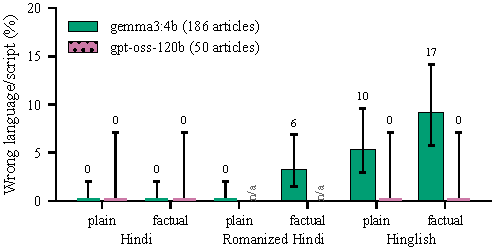
\includegraphics[width=\columnwidth]{fig_wrong_language}
  \caption{Share of summaries in the wrong language or script (95\% Wilson intervals; numbers above bars are counts). gpt-oss-120b was run on 50 articles for \cond{hi} and \cond{hinglish} only.}
  \label{fig:wronglang}
\end{figure}

\begin{figure}[t]
  \centering
  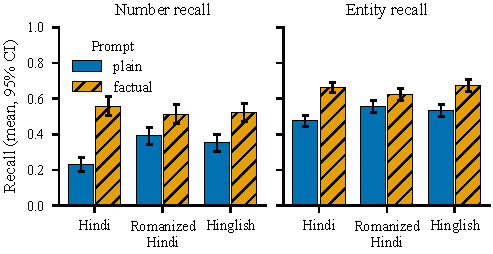
\includegraphics[width=\columnwidth]{fig_recall_by_condition}
  \caption{Number and entity recall of gemma3:4b summaries by condition and prompt (mean with 95\% bootstrap CI; summaries in the wrong language excluded).}
  \label{fig:recall}
\end{figure}

\begin{table*}[t]
\centering
\caption{gemma3:4b, all 186 articles: means over summaries that passed the language check ($n$). P/R = precision/recall. 95\% bootstrap CIs are in \texttt{results/summary\_table\_gemma3\_4b.csv}. NLI is comparable only within a condition.}
\label{tab:main}
\setlength{\tabcolsep}{4.5pt}
\begin{tabular}{@{}llrcccccccccc@{}}
\toprule
Condition & Prompt & $n$ & Num P & Num R & Ent P & Ent R & NLI chunk & NLI window & ROUGE-2 & BERTScore & Words \\
\midrule
\multirow{2}{*}{\cond{hi}}       & plain   & 186 & 0.979 & 0.230 & 0.974 & 0.475 & 0.742 & 0.745 & 0.141 & 0.749 & 73.9 \\
                                 & factual & 186 & 0.970 & 0.556 & 0.994 & 0.661 & 0.613 & 0.727 & 0.259 & 0.787 & 78.6 \\
\multirow{2}{*}{\cond{hi-rom}}   & plain   & 186 & 0.999 & 0.390 & 0.995 & 0.553 & 0.475 & 0.713 & 0.388 & 0.788 & 80.9 \\
                                 & factual & 180 & 1.000 & 0.513 & 1.000 & 0.624 & 0.454 & 0.708 & 0.440 & 0.792 & 84.7 \\
\multirow{2}{*}{\cond{hinglish}} & plain   & 176 & 0.981 & 0.352 & 0.979 & 0.534 & 0.511 & 0.632 & 0.248 & 0.746 & 83.3 \\
                                 & factual & 169 & 1.000 & 0.523 & 0.997 & 0.675 & 0.397 & 0.647 & 0.419 & 0.786 & 87.5 \\
\bottomrule
\end{tabular}
\end{table*}

\begin{table*}[t]
\centering
\caption{gpt-oss-120b vs.\ gemma3:4b on the same 50 articles. Wrong-language rate over all 50 summaries per cell; all other columns are means over the $n$ rows where both models answered in the right language.}
\label{tab:models}
\setlength{\tabcolsep}{4pt}
\begin{tabular}{@{}lllrrcccccccc@{}}
\toprule
Condition & Prompt & Model & Wrong lang. & $n$ & Num P & Num R & Ent P & Ent R & NLI chunk & NLI window & ROUGE-L & Words \\
\midrule
\multirow{4}{*}{\cond{hi}} & \multirow{2}{*}{plain} & gemma3:4b & 0\% & 50 & 0.926 & 0.197 & 0.985 & 0.461 & 0.729 & 0.739 & 0.212 & 75.3 \\
 & & gpt-oss-120b & 0\% & 50 & 0.958 & 0.465 & 0.987 & 0.543 & 0.669 & 0.624 & 0.223 & 76.2 \\
 & \multirow{2}{*}{factual} & gemma3:4b & 0\% & 50 & 0.987 & 0.499 & 1.000 & 0.657 & 0.625 & 0.721 & 0.297 & 78.2 \\
 & & gpt-oss-120b & 0\% & 50 & 0.996 & 0.651 & 0.980 & 0.729 & 0.566 & 0.643 & 0.382 & 96.2 \\
\midrule
\multirow{4}{*}{\cond{hinglish}} & \multirow{2}{*}{plain} & gemma3:4b & 10\% & 45 & 0.994 & 0.311 & 0.962 & 0.590 & 0.576 & 0.623 & 0.312 & 82.7 \\
 & & gpt-oss-120b & 0\% & 45 & 1.000 & 0.457 & 0.987 & 0.605 & 0.510 & 0.545 & 0.309 & 82.8 \\
 & \multirow{2}{*}{factual} & gemma3:4b & 14\% & 43 & 1.000 & 0.504 & 0.996 & 0.675 & 0.445 & 0.642 & 0.428 & 87.0 \\
 & & gpt-oss-120b & 0\% & 43 & 1.000 & 0.660 & 1.000 & 0.742 & 0.422 & 0.569 & 0.429 & 99.1 \\
\bottomrule
\end{tabular}
\end{table*}

\begin{figure}[t]
  \centering
  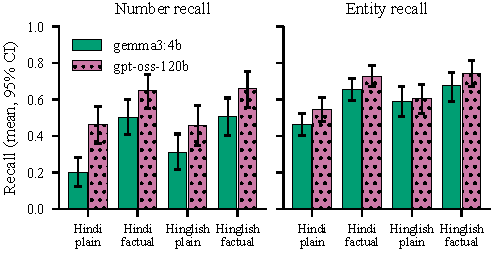
\includegraphics[width=\columnwidth]{fig_model_recall}
  \caption{Number and entity recall of gemma3:4b and gpt-oss-120b on the same 50 articles (188 summaries where both models answered in the right language; 95\% bootstrap CI).}
  \label{fig:models}
\end{figure}

\begin{figure}[t]
  \centering
  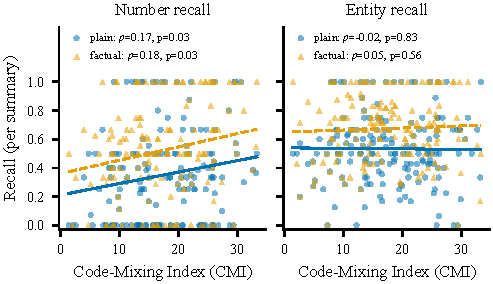
\includegraphics[width=\columnwidth]{fig_cmi_recall}
  \caption{Per-summary recall vs.\ Code-Mixing Index of the source, \cond{hinglish} condition, gemma3:4b, with least-squares lines and Spearman $\rho$.}
  \label{fig:cmi}
\end{figure}

\begin{figure}[t]
  \centering
  \fbox{\parbox[c][3.5cm][c]{0.9\columnwidth}{\centering
    \todo{Figure: agreement of each automatic metric with human labels\\(AUC, faithful vs.\ error, 95\% CI).\\Generated by \texttt{src.analysis.make\_figures} once\\\texttt{src.eval.merge\_annotations} has run.}}}
  \caption{\todo{Metric--human agreement.}}
  \label{fig:agreement}
\end{figure}

\section{Error Analysis}
\label{sec:errors}

\paragraph{Error types} Error types were given by three of the five annotators (A1, A4, A5; A2 and A3 gave labels only), so 21 of the 34 erroneous summaries have a final type (Fig.~\ref{fig:errortypes}b). \emph{Meaning} errors, in which correct names and numbers are put in a wrong relation, dominate: 14 of 21 final types, and 22 of the 32 typed error labels of the three annotators. Omissions that make a summary misleading follow (4 of 21); number, entity and added-information errors occur once each. This matches the automatic results: invented names and numbers are rare, so the precision metrics are at the ceiling, while the errors humans find are about relations. Thirty-three of the 34 erroneous summaries have perfect number and entity precision.

\paragraph{Relation errors that the automatic metrics pass} The three major errors below were labelled by the annotators; each has number and entity precision 1.0 (or no number), and each passes NLI-window.
\begin{itemize}
  \item \emph{Outcome reversal} (\cond{hinglish}, plain): a rain-shortened England--Pakistan ODI was abandoned with Pakistan on 46 for 1, but the summary says ``Pakistan ne 46 run mein ek wicket loss ke saath match jeeta'' (Pakistan won the match). NLI-window 0.80, NLI-chunk 0.28.
  \item \emph{Outcome reversal} (\cond{hinglish}, plain): an India--England Test was drawn with India on 391/9, but the summary says India ``England ko khatam kar diya'' (finished England off), although all scores, Root's 154 and Anderson's man-of-the-match award are copied correctly. NLI-window 0.75, NLI-chunk 0.28.
  \item \emph{Role reversal} (\cond{hi-rom}, factual): in the source, George Fernandes supports the vegetable vendors protesting against Reliance and condemns the police brutality against them; the summary says he \emph{supported} the police's brutal treatment of the vendors and attributes to him an assurance of full protection for Reliance Fresh that, in the source, was given by the Chief Minister. NLI-window 0.66, NLI-chunk 0.52.
\end{itemize}
The same pattern appears outside the labelled set. In a \cond{hi} plain summary, gemma3:4b writes that Boeing launched the Dreamliner in 1995; the source gives 1995 as the launch year of the Boeing 777. Both the number and the name occur in the source, so number and entity precision are 1.0, and NLI scores the summary 0.76 (chunk) and 0.82 (window).

\paragraph{Errors that the precision metrics do catch} The few non-relation errors are caught by the script-independent checks. A \cond{hi-rom} plain summary says ``char lakh'' (4 lakh) children run away from home every year, where the source has 4 lakh 40 thousand; the parsed values differ, so number precision drops to 0.86. A \cond{hi} plain summary of the India--England Test writes the full name ``James Anderson'' (in Devanagari) where the source names only ``Anderson''; the first name is correct world knowledge but not in the article, and entity precision drops to 0.83. Under our guidelines both count as errors, the second as added information.

\paragraph{Script-conversion errors} Romanization loses information that the model sometimes restores wrongly. In the \cond{hi-rom} version of an article on the Bihar floods, \dev{बाढ़} (\emph{baadh}, flood) is written \emph{barh}, because our romanization does not mark vowel length. Asked for a factual summary, gemma3:4b answered in Devanagari and back-transliterated \emph{barh} as \dev{बारह} (\emph{baarah}, twelve) four times, e.g.\ ``\dev{बारह पीड़ितों को भूखा नहीं रहने दिया जाएगा}'' (``the \emph{twelve} victims will not be left hungry'' instead of ``the flood victims''). The summary failed the script check, so it was excluded from the factuality metrics and counts only towards the wrong-language rate; had it been scored, the number parser would have read \dev{बारह} as an invented 12.

\paragraph{Metric failure cases} Exact number-word lists also cause false positives: the surname ``Das'' is read as 10 (\emph{das}). In the labelled set, however, the precision metrics never flagged a faithful summary; the main failure is the opposite one, missed relation errors. NLI fails in both directions: NLI-window passes 31 of 34 erroneous summaries, and NLI-chunk scores 13 of 26 faithful summaries below 0.5.

\begin{figure}[t]
  \centering
  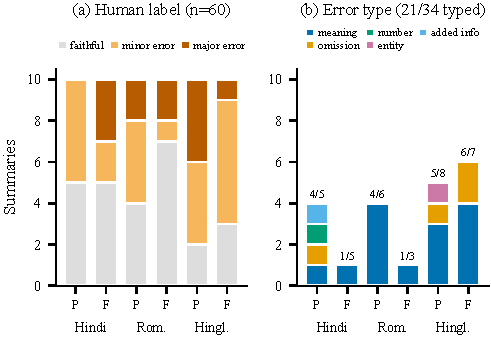
\includegraphics[width=\columnwidth]{fig_error_types}
  \caption{(a) Final human label of the 60 labelled gemma3:4b summaries (10 per condition and prompt; P = plain, F = factual). (b) Error type of the erroneous summaries that have one (typed / all errors above each bar); two of the five annotators gave no error types.}
  \label{fig:errortypes}
\end{figure}

\section{Conclusion}
\label{sec:conclusion}

% OUTLINE
\todo{Write after Results and Error Analysis.}

\begin{itemize}
  \item Summary of findings: language control as the first failure mode for a small model on Romanized/Hinglish input; precision at ceiling; factual prompt raises coverage; \todo{human-label headline}.
  \item What practitioners should measure: wrong-language rate, script-independent number/entity checks, and human labels for relation errors.
  \item Limitations (synthetic Hinglish, one small and one large model, 60 labelled summaries).
  \item Future work: naturally occurring Hinglish news, QA-based metrics for code-mixed text, more models.
\end{itemize}


\section*{Acknowledgment}
We thank Dr.\ Geetanjali Singh, Bennett University, for her guidance on this CSET~346 Natural Language Processing project.

\bibliographystyle{IEEEtran}
\bibliography{references}

\end{document}
